\chapter{Managing the Kernel}

\section{Understanding the Modular Structure of the Kernel}	
The primary responsibility of the Linux Kernel is addressing the hardware and managing it. By default the kernel contains every functionality required to address the available hardware. 

\begin{figure}[H]
	\centering
	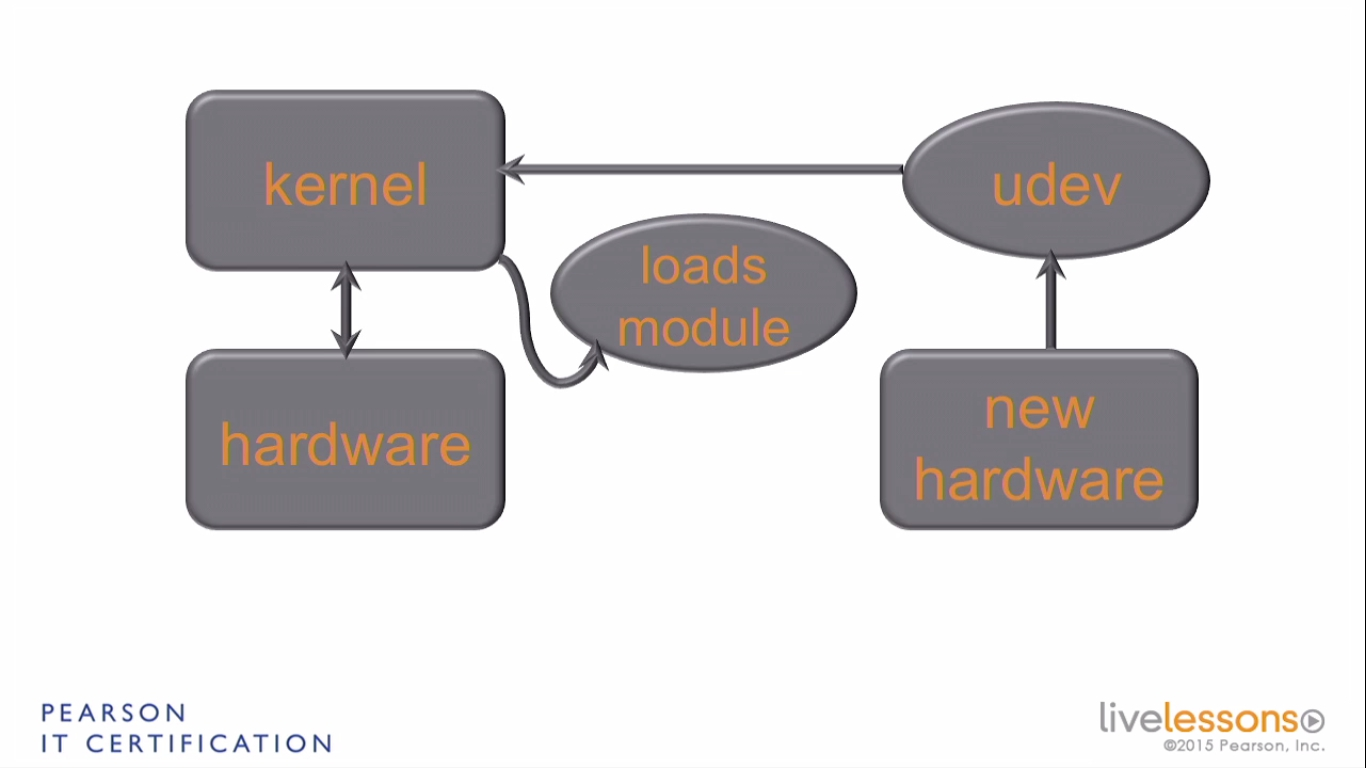
\includegraphics[width=0.9\linewidth]{Mod3/chapters/3.17.a}
	\caption{Modular structure of the Kernel}
	\label{fig:3}
\end{figure}

When a new hardware is added, the \textbf{udev} process is awoken to initialize the new hardware by communicating with the kernel and providing it with all the necessary information about the device. In turn, the kernel will load the module specific to that new hardware and initialize it so that the user can start using it. 

	\section{Working with Kernel Modules}
The linux kernel works with modules to only load those modules which provided a required functionality. Thus, these kernels are very lean since only the functionalities being used are kept. 

\subsection{Viewling loaded Kernel Modules}
\vspace{-5pt}
The \verb|lsmod| command shows us all the kernel module that have been loaded. 

\vspace{-15pt}
\begin{minted}{console}
# lsmod
Module                  Size  Used by
nls_utf8               12557  1 
isofs                  39844  1 
fuse                   91874  3 
xt_CHECKSUM            12549  1 
ipt_MASQUERADE         12678  3 
...
dm_region_hash         20813  1 dm_mirror
dm_log                 18411  2 dm_region_hash,dm_mirror
dm_mod                123303  14 dm_log,dm_mirror
\end{minted}
\vspace{-10pt}

\noindent
The provided data is the name and size of the module followed by the number of programs currently using the module. In older versions of linux it was required to manually load modules to access certain functionalities. Modern linux distros don't require this. The \textbf{udev} process takes care of loading modules automatically. The activity of this process can be monitored using the \verb|udevadm monitor| command.

\vspace{-15pt}
\begin{minted}{console}
monitor will print the received events for:
UDEV - the event which udev sends out after rule processing
KERNEL - the kernel uevent
\end{minted}
\vspace{-10pt}

\noindent
Now if we were to attach a pen drive (and then remove it) then that'd trigger the following:

\vspace{-15pt}
\begin{minted}{bash}
KERNEL[15445.778458] add      /devices/pci0000:00/0000:00:11.0/0000:02:03.0/usb1/1-1 (usb)
KERNEL[15445.786957] add      /devices/pci0000:00/0000:00:11.0/0000:02:03.0/usb1/1-1/1-1:1.0 (usb)
UDEV  [15445.830980] add      /devices/pci0000:00/0000:00:11.0/0000:02:03.0/usb1/1-1 (usb)
KERNEL[15445.851667] add      /module/usb_storage (module)
UDEV  [15445.877116] add      /module/usb_storage (module)
...

KERNEL[15893.875998] add      /module/fat (module)
KERNEL[15893.876022] add      /kernel/slab/fat_cache (slab)
KERNEL[15893.876030] add      /kernel/slab/fat_inode_cache (slab)
KERNEL[15893.876037] add      /module/vfat (module)
UDEV  [15893.878942] add      /module/fat (module)
UDEV  [15893.878962] add      /kernel/slab/fat_cache (slab)
UDEV  [15893.878969] add      /kernel/slab/fat_inode_cache (slab)
UDEV  [15893.879002] add      /module/vfat (module)

...
UDEV  [15462.218411] remove   /devices/pci0000:00/0000:00:11.0/0000:02:03.0/usb1/1-1 (usb)
KERNEL[15462.232117] remove   /host3/target3:0:0 (scsi)
UDEV  [15462.232957] remove   /host3/target3:0:0 (scsi)
\end{minted}
\vspace{-10pt}

\noindent
The moment new hardware is detected, it generates an event which is then received by udev to respond appropriately. The insertion of the pen drive (usb key) into the usb slot triggered the udev process to load the \textit{fat} and \textit{vfat} modules [Lines \verb|8-15|].

However, when the USB key is detached, the modules aren't unloaded. This can be verified by the presence of both \textit{fat \& vfat} modules in the output of:

\vspace{-15pt}
\begin{minted}{console}
# lsmod | grep fat
vfat                   17461  0 
fat                    65950  1 vfat
\end{minted}
\vspace{-10pt}	

\subsection{Modprobe}
\vspace{-5pt}
The \verb|modprobe| command is used to load kernel modules  manually. With the \verb|-r| option, the command \verb|modprobe -r| can also be used to unload kernel modules. We can remove the vfat module by:

\vspace{-15pt}
\begin{minted}{console}
# modprobe -r vfat
# lsmod | grep fat
# 
\end{minted}
\vspace{-10pt}	

\noindent
Note that the \textit{fat} kernel module was loaded while loading the \textit{vfat} kernel module and when the \textit{vfat} module was unloaded by \verb|modprobe|, it's dependency, \textit{fat} module was also unloaded. Thus, \verb|modprobe| also manages loading and unloading the dependencies. To load the \textit{vfat} module again, we use:

\vspace{-15pt}
\begin{minted}{console}
# modprobe vfat
# lsmod | grep fat
vfat                   17461  0 
fat                    65950  1 vfat
\end{minted}
\vspace{-10pt}

\noindent
Normally, this is something we have to rarely do, since the udev process does its work so well once the kernel has detected the hardware. However, this is extremely useful for situations where the kernel module has been edited/updated manually and needs to be reloaded. 

\section{Modifying the Kernel module behavior through modprobe}
The information about any specific kernel module can be obtained through the \verb|modinfo| command. 

\vspace{-15pt}
\begin{minted}{console}
# modinfo e1000
filename:       /lib/modules/3.10.0-693.11.1.el7.x86_64/kernel/drivers/net/ethernet/intel/e1000/e1000.ko.xz
version:        7.3.21-k8-NAPI
license:        GPL
description:    Intel(R) PRO/1000 Network Driver
author:         Intel Corporation, <linux.nics@intel.com>
rhelversion:    7.4
srcversion:     9E0A112E5D47C996E7C4A58
alias:          pci:v00008086d00002E6Esv*sd*bc*sc*i*
...
alias:          pci:v00008086d00001001sv*sd*bc*sc*i*
alias:          pci:v00008086d00001000sv*sd*bc*sc*i*
depends:        
intree:         Y
vermagic:       3.10.0-693.11.1.el7.x86_64 SMP mod_unload modversions 
signer:         CentOS Linux kernel signing key
sig_key:        61:B8:E8:7B:84:11:84:F6:2F:80:D6:07:79:AB:69:2A:49:D8:3B:AF
sig_hashalgo:   sha256
parm:           TxDescriptors:Number of transmit descriptors (array of int)
parm:           RxDescriptors:Number of receive descriptors (array of int)
parm:           Speed:Speed setting (array of int)
parm:           Duplex:Duplex setting (array of int)
parm:           AutoNeg:Advertised auto-negotiation setting (array of int)
...
parm:           copybreak:Maximum size of packet that is copied to a new buffer on receive (uint)
parm:           debug:Debug level (0=none,...,16=all) (int)
\end{minted}
\vspace{-10pt}

\noindent
What's really useful for us is the \textit{parm} information towards the end of the kernel module. While not every kernel module has them, many kernel module do provide the option to set parameters. Thus, the \verb|modinfo| command gives us a list of all the parameters that can be set for a kernel module. 

Now, we can see the information about the parameters that are available for the \textit{cdrom} module:

\vspace{-15pt}
\begin{minted}{console}
# modinfo cdrom
filename:       /lib/modules/3.10.0-693.11.1.el7.x86_64/kernel/drivers/cdrom/cdrom.ko.xz
license:        GPL
rhelversion:    7.4
srcversion:     BE3BD0D17D080229D55B173
depends:        
intree:         Y
vermagic:       3.10.0-693.11.1.el7.x86_64 SMP mod_unload modversions 
signer:         CentOS Linux kernel signing key
sig_key:        61:B8:E8:7B:84:11:84:F6:2F:80:D6:07:79:AB:69:2A:49:D8:3B:AF
sig_hashalgo:   sha256
parm:           debug:bool
parm:           autoclose:bool
parm:           autoeject:bool
parm:           lockdoor:bool
parm:           check_media_type:bool
parm:           mrw_format_restart:bool
\end{minted}
\vspace{-10pt}

\noindent
An interesting example of a parameter is the \textit{lockdoor} parameter, which when enabled locks the cd tray when the device is mounted. In case of these boolean variables, the value \verb|0 = false;	1 = true|. If however, we try to remove a kernel module that's being used, we get the message:

\vspace{-15pt}
\begin{minted}{console}
# modprobe -r cdrom
modprobe: FATAL: Module cdrom is in use.
\end{minted}
\vspace{-10pt}

\noindent
If the cdrom weren't in use, the command to set the parameter (stop locking the disk tray when the cdrom is mounted) would be: 

\vspace{-15pt}
\begin{minted}{console}
# modprobe cdrom lockdoor=0
\end{minted}
\vspace{-10pt}

\subsection{Setting kernel module parameters on older Linux versions}
There was only one entry point for setting the kernel module parameters on older versions of Linux : \verb|/etc/modprobe.conf|. However, RHEL 7 onwards, this is no longer the case. There are a couple of extra locations for modifying the kernel module parameters. 

The folder \verb|/lib/modprobe.d| contains many configuration files. These files contain the default settings for their respective kernel modules. The files are dropped here by the RPMs during installation. Typically, we should avoid any modification in this folder. 

To modify the kernel parameters we should choose a different directory: \verb|/etc/modprobe.d|. There is an excellent manpage for the modprobe.d directory, which contains the format for specifying the parameters:

\vspace{-15pt}
\begin{minted}{bash}
options modulename option...
\end{minted}
\vspace{-10pt}

\noindent
Thus, to set the kernel parameter for the lockdoor on cdrom to false, we need to make a file: \verb|/etc/modprobe.d/cdrom.conf| which contains just one line:

\vspace{-15pt}
\begin{minted}{bash}
options cdrom lockdoor=0
\end{minted}
\vspace{-10pt}

\noindent
Since in our case, we can't reload the kernel module since it's in use, the only way to ensure that it works is by rebooting the server with \verb|reboot now|. Finding out if it worked might be problematic on a live system. 

For certain modules, we can go to the \verb|/sys/module| directory which contains a sub-directory for every kernel module that's currently loaded. We would want to look for a file called \verb|parameters| that sits in the directory for that module name, and check to see what value is set. However, the cdrom module has no such file. 

Next, we can check the wih the \verb|dmesg| command, after filtering it appropriately. Then we filter out the irrelevant stuff with the \verb|grep| command. The grep command can be provided an option \verb|-A| which is followed immediately by the number of lines starting from the matching line should be printed. 

\vspace{-15pt}
\begin{minted}{console}
# dmesg | grep cdrom
[    2.516616] cdrom: Uniform CD-ROM driver Revision: 3.20
# dmesg | grep -A5 cdrom
[    2.516616] cdrom: Uniform CD-ROM driver Revision: 3.20
[    2.516931] sr 2:0:0:0: Attached scsi CD-ROM sr0
[    2.818361] e1000 0000:02:01.0 eth0: (PCI:66MHz:32-bit) 00:0c:29:d6:73:d0
[    2.818369] e1000 0000:02:01.0 eth0: Intel(R) PRO/1000 Network Connection
[    3.137847] random: crng init done
[    3.666093] SGI XFS with ACLs, security attributes, no debug enabled
\end{minted}
\vspace{-10pt}

\section{Tuning kernel behavior through proc}
The Linux kernel provides an easy to use interface to optimize kernel parameters, called \textbf{proc}. To use it, we have to go to the \verb|/proc| file system. In there we can find current status information about the kernel, and also a \verb|/proc/sys| directory that helps us optimize kernel parameters. 

There are several files that convey kernel status information, such as the \verb|/proc/cpuinfo| file that helped us detect if the virtualization flag (\textit{vmx}) was set for the processor. There is also the \verb|/proc/partitions| file that shows us the kernel partition table contents. The \verb|/proc/meminfo| file gives us detailed information about the memory. 

In the \verb|/proc/sys| directory, there is a subdirectory for every interface offered by the kernel. Some of the most important ones are : \textbf{kernel} - to optimize core kernel functionality, \textbf{net} - for networking and \textbf{vm} - concerning virtual memory management.

If the module has to be loaded, then the parameters should be edited with \verb|/etc/modprobe.d/<moduleName>.conf|. However, if they're a part of the main kernel, then there's a chance that there's a \verb|sysctl| setting available for it. In that case, it can be edited via the proc file system. All sysctl settings are available under \verb|/proc/sys| directory. 

If we go to the \verb|/proc/sys/kernel| folder, we can see that there are a lot of parameters that the kernel is using. While some of the parameters are quite advanced, some are simple and provide useful information such as the \textit{osrelease and hostname} files. 

\vspace{-15pt}
\begin{minted}{console}
# cat /proc/sys/kernel/osrelease 
3.10.0-693.11.1.el7.x86_64
# cat /proc/sys/kernel/hostname 
vmPrime.somuVMnet.local
\end{minted}
\vspace{-10pt}

\noindent
We can also change the parameters here. For example, in the \verb|/proc/sys/net/ipv4| directory, there is a file for a parameter called \textit{ip\_forward}. 

\vspace{-15pt}
\begin{minted}{console}
# cat ip_forward
1
\end{minted}
\vspace{-10pt}

\noindent
This means that the system is configured to forward packets, i.e., the system is configured as a router. If we want to change this behavior, and want to turn that parameter off, we just use the command \verb|echo 0 > ip\_forward|. Note that changing parameters this way is not persistent. 

In the \verb|/proc/sys/vm| directory, there is a file for the swappiness parameter, i.e., the willingness to swap or store a file on the hard disk from the RAM when it's no longer needed. This parameter accepts values between $0$ to $100$ and if we increase the swappiness, we make the kernel swap out data to disk faster. 

An important point of note is that the system parameters in this directory are really advanced, and we should only change the values here if we know exactly what we're doing. This is not a place for \textit{experimentation}, as it may even cause boot to fail.

\section{Using sysctl}
To make the changes that we've made persistent, we have to tune \textbf{sysctl}. 

\subsection{sysctl command}
The \verb|sysctl| command is used to configure the kernel parameters at runtime. The \verb|sysctl -a| command gives us a list of all the tunable options that are currently set. 

\vspace{-15pt}
\begin{minted}{console}
# sysctl -a
abi.vsyscall32 = 1
crypto.fips_enabled = 0
debug.exception-trace = 1
debug.kprobes-optimization = 1
debug.panic_on_rcu_stall = 0
dev.cdrom.autoclose = 1
dev.cdrom.autoeject = 0
...
vm.vfs_cache_pressure = 100
vm.zone_reclaim_mode = 0
\end{minted}
\vspace{-10pt}

\noindent
This list is also greppable, and thus, we can easily find the parameter we're looking for. 

\vspace{-15pt}
\begin{minted}{console}
# sysctl -a | grep ip_forward
sysctl: reading key "net.ipv6.conf.all.stable_secret"
sysctl: reading key "net.ipv6.conf.default.stable_secret"
sysctl: reading key "net.ipv6.conf.ens33.stable_secret"
sysctl: reading key "net.ipv6.conf.lo.stable_secret"
sysctl: reading key "net.ipv6.conf.virbr0.stable_secret"
sysctl: reading key "net.ipv6.conf.virbr0-nic.stable_secret"
net.ipv4.ip_forward = 0
net.ipv4.ip_forward_use_pmtu = 0
\end{minted}
\vspace{-10pt}

\noindent
The names of the parameters shown here correspond to a file of the same name in the \verb|/proc/sys/| directory. Thus, the \verb|net.ipv4.ip_forward| parameter can be set using the file \verb|/proc/sys/net/ipv4/ip_forward| file. 

Upon booting the sysctl process reads a bunch of configuration files to appropriately set the kernel parameters. In earlier versions, there used to be only one config file: \verb|/etc/sysctl.conf|, but on RHEL 7 it's empty. For custom settings, the \verb|/etc/sysctl.d/<name>.conf| files should be used. The default sysctl config is loaded from the \verb|/usr/lib/sysctl.d/| files. The contents of that directory is:

\vspace{-15pt}
\begin{minted}{console}
# ls /usr/lib/sysctl.d/
00-system.conf  10-default-yama-scope.conf  50-default.conf  60-libvirtd.conf
\end{minted}
\vspace{-10pt}

\noindent
The numbers in front of the file names just ensure that the config settings are read from the files in order. So, \textit{00-system.conf} will be read before \textit{60-libvirtd.conf}. This gives a cascading effect, and if a setting is saved in multiple files then the last file to be read contains the value that'll be used. 

Now, if we want our computer to be able to forward IP packets like a router, we edit the file \verb|/etc/sysctl.d/50-ipforward.conf|:

\vspace{-15pt}
\begin{minted}{bash}
net.ipv4.ip_forward = 1
\end{minted}
\vspace{-10pt}

\noindent
After the next reboot, the system will be able to route ip packets. There are certain tools that can write directly to the sysctl config files, but they should be avoided, since to verify that these work, we have to echo their values from the \verb|/proc| file system. Then all we need to do is restart the system, and since the tunable is a part of sysctl system, the parameters will be applied at next boot.

	\section{Updating the kernel}
The command to update the kernel is:

\vspace{-15pt}
\begin{minted}{console}
# yum update kernel
\end{minted}
\vspace{-10pt}

\noindent
If the kernel has already been downloaded, we could use either of the commands below:

\vspace{-15pt}
\begin{minted}{console}
# yum localinstall <kernelName>.rpm
# rpm -Uvh <kernelName>.rpm
\end{minted}
\vspace{-10pt}

In any case, the old kernel is not overwritten during the update, and thus it can still be booted, as both are added to grub. 